% xcolor and define colors -------------------------
\usepackage{xcolor}

% https://www.viget.com/articles/color-contrast/
\definecolor{purple}{HTML}{5601A4}
\definecolor{navy}{HTML}{0D3D56}
\definecolor{ruby}{HTML}{9a2515}
\definecolor{alice}{HTML}{107895}
\definecolor{daisy}{HTML}{EBC944}
\definecolor{coral}{HTML}{F26D21}
\definecolor{kelly}{HTML}{829356}
\definecolor{cranberry}{HTML}{E64173}
\definecolor{jet}{HTML}{131516}
\definecolor{asher}{HTML}{555F61}
\definecolor{slate}{HTML}{314F4F}

% Mixtape Sessions
\definecolor{picton-blue}{HTML}{00b7ff}
\definecolor{violet-red}{HTML}{ff3881}
\definecolor{sun}{HTML}{ffaf18}
\definecolor{electric-violet}{HTML}{871EFF}

\newcommand\pictonBlue[1]{{\color{picton-blue}#1}}
\newcommand\sun[1]{{\color{sun}#1}}
\newcommand\electricViolet[1]{{\color{electric-violet}#1}}
\newcommand\violetRed[1]{{\color{violet-red}#1}}

\newcommand\bgPictonBlue[1]{{\colorbox{picton-blue!20!white}{#1}}}
\newcommand\bgSun[1]{{\colorbox{sun!20!white}{#1}}}
\newcommand\bgElectricViolet[1]{{\colorbox{electric-violet!20!white}{#1}}}
\newcommand\bgVioletRed[1]{{\colorbox{violet-red!20!white}{#1}}}

\def\code#1{\texttt{#1}}

% Main theme colors
\definecolor{accent}{HTML}{00b7ff}
\definecolor{accent2}{HTML}{871EFF}
\definecolor{gray100}{HTML}{f3f4f6}
\definecolor{gray800}{HTML}{1F292D}


% Beamer Options -------------------------------------

% Background
\setbeamercolor{background canvas}{bg = white}

% Change text margins
\setbeamersize{text margin left = 15pt, text margin right = 15pt} 

% \alert
\setbeamercolor{alerted text}{fg = accent2}

% Frame title
\setbeamercolor{frametitle}{bg = white, fg = jet}
\setbeamercolor{framesubtitle}{bg = white, fg = accent}
\setbeamerfont{framesubtitle}{size = \small, shape = \itshape}

% Block
\setbeamercolor{block title}{fg = white, bg = accent2}
\setbeamercolor{block body}{fg = gray800, bg = gray100}

% Title page
\setbeamercolor{title}{fg = gray800}
\setbeamercolor{subtitle}{fg = accent}

%% Custom \maketitle and \titlepage
\setbeamertemplate{title page}
{
    %\begin{centering}
        \vspace{20mm}
        {\Large \usebeamerfont{title}\usebeamercolor[fg]{title}\inserttitle}\\
        {\large \itshape \usebeamerfont{subtitle}\usebeamercolor[fg]{subtitle}\insertsubtitle}\\ \vspace{10mm}
        {\insertauthor}\\
        {\color{asher}\small{\insertdate}}\\
    %\end{centering}
}

% Table of Contents
\setbeamercolor{section in toc}{fg = accent!70!jet}
\setbeamercolor{subsection in toc}{fg = jet}

% Button 
\setbeamercolor{button}{bg = accent}

% Remove navigation symbols
\setbeamertemplate{navigation symbols}{}

% Table and Figure captions
\setbeamercolor{caption}{fg=jet!70!white}
\setbeamercolor{caption name}{fg=jet}
\setbeamerfont{caption name}{shape = \itshape}

% Bullet points

%% Fix spacing between items
\let\olditemize=\itemize 
\let\endolditemize=\enditemize 
\renewenvironment{itemize}{\vspace{0.25em}\olditemize \itemsep0.25em}{\endolditemize}

%% Fix left-margins
\settowidth{\leftmargini}{\usebeamertemplate{itemize item}}
\addtolength{\leftmargini}{\labelsep}

%% enumerate item color
\setbeamercolor{enumerate item}{fg = accent}
\setbeamerfont{enumerate item}{size = \small}
\setbeamertemplate{enumerate item}{\insertenumlabel.}

%% itemize
\setbeamercolor{itemize item}{fg = accent!70!white}
\setbeamerfont{itemize item}{size = \small}
\setbeamertemplate{itemize item}[circle]

%% right arrow for subitems
\setbeamercolor{itemize subitem}{fg = accent!60!white}
\setbeamerfont{itemize subitem}{size = \small}
\setbeamertemplate{itemize subitem}{$\rightarrow$}

\setbeamertemplate{itemize subsubitem}[square]
\setbeamercolor{itemize subsubitem}{fg = jet}
\setbeamerfont{itemize subsubitem}{size = \small}








% Links ----------------------------------------------

\usepackage{hyperref}
\hypersetup{
  colorlinks = true,
  linkcolor = accent2,
  filecolor = accent2,
  urlcolor = accent2,
  citecolor = accent2,
}


% Line spacing --------------------------------------
\usepackage{setspace}
\setstretch{1.35}


% \begin{columns} -----------------------------------
\usepackage{multicol}


% Fonts ---------------------------------------------
% Beamer Option to use custom fonts
\usefonttheme{professionalfonts}

% \usepackage[utopia, smallerops, varg]{newtxmath}
% \usepackage{utopia}
\usepackage[sfdefault,light]{roboto}

% Small adjustments to text kerning
\usepackage{microtype}



% Remove annoying over-full box warnings -----------
\vfuzz2pt 
\hfuzz2pt


% Table of Contents with Sections
\setbeamerfont{myTOC}{series=\bfseries, size=\Large}
\AtBeginSection[]{
        \frame{
            \frametitle{Roadmap}
            \tableofcontents[current]   
        }
    }


% Tables -------------------------------------------
% Tables too big
% \begin{adjustbox}{width = 1.2\textwidth, center}
\usepackage{adjustbox}
\usepackage{array}
\usepackage{threeparttable, booktabs, adjustbox}
    
% Fix \input with tables
% \input fails when \\ is at end of external .tex file
\makeatletter
\let\input\@@input
\makeatother

% Tables too narrow
% \begin{tabularx}{\linewidth}{cols}
% col-types: X - center, L - left, R -right
% Relative scale: >{\hsize=.8\hsize}X/L/R
\usepackage{tabularx}
\newcolumntype{L}{>{\raggedright\arraybackslash}X}
\newcolumntype{R}{>{\raggedleft\arraybackslash}X}
\newcolumntype{C}{>{\centering\arraybackslash}X}

% Figures

% \imageframe{img_name} -----------------------------
% from https://github.com/mattjetwell/cousteau
\newcommand{\imageframe}[1]{%
    \begin{frame}[plain]
        \begin{tikzpicture}[remember picture, overlay]
            \node[at = (current page.center), xshift = 0cm] (cover) {%
                \includegraphics[keepaspectratio, width=\paperwidth, height=\paperheight]{#1}
            };
        \end{tikzpicture}
    \end{frame}%
}

% subfigures
\usepackage{subfigure}


% Highlight slide -----------------------------------
% \begin{transitionframe} Text \end{transitionframe}
% from paulgp's beamer tips
\newenvironment{transitionframe}{
    \setbeamercolor{background canvas}{bg=accent!40!black}
    \begin{frame}\color{accent!10!white}\LARGE\centering
}{
    \end{frame}
}


% Table Highlighting --------------------------------
% Create top-left and bottom-right markets in tabular cells with a unique matching id and these commands will outline those cells
\usepackage[beamer,customcolors]{hf-tikz}
\usetikzlibrary{calc}
\usetikzlibrary{fit,shapes.misc}

% To set the hypothesis highlighting boxes red.
\newcommand\marktopleft[1]{%
    \tikz[overlay,remember picture] 
        \node (marker-#1-a) at (0,1.5ex) {};%
}
\newcommand\markbottomright[1]{%
    \tikz[overlay,remember picture] 
        \node (marker-#1-b) at (0,0) {};%
    \tikz[accent!80!jet, ultra thick, overlay, remember picture, inner sep=4pt]
        \node[draw, rectangle, fit=(marker-#1-a.center) (marker-#1-b.center)] {};%
}


% DAGS ----------------------------------------------
\usepackage{tikz}
\usetikzlibrary{shapes,decorations,arrows,calc,arrows.meta,fit,positioning}
% Tikz settings optimized for causal graphs.
\tikzset{
    -Latex,auto,node distance =1 cm and 1 cm,semithick,
    state/.style ={ellipse, draw, minimum width = 0.7 cm},
    point/.style = {circle, draw, inner sep=0.04cm,fill,node contents={}},
    bidirected/.style={Latex-Latex,dashed},
    el/.style = {inner sep=2pt, align=left, sloped}
}


% Beamer tricks -------------------------------------
% Make \pause work in align environments
\makeatletter
\renewrobustcmd{\beamer@@pause}[1][]{%
  \unless\ifmeasuring@%
  \ifblank{#1}%
    {\stepcounter{beamerpauses}}%
    {\setcounter{beamerpauses}{#1}}%
  \onslide<\value{beamerpauses}->\relax%
  \fi%
}
\makeatother


\title [Nonparametrics]{Nonparametrics and Local Methods: Splines}
\author{C.Conlon}
\institute{Applied Econometrics}
\date{\today}
\setbeamerfont{equation}{size=\tiny}
\begin{document}

\begin{frame}
\titlepage
\end{frame}
\begin{frame}{Polynomial Basis}
Again consider the following relationship:
\begin{align*}
y_i = f(x_i) + \epsilon_i
\end{align*}
One approach is to approximate $f(x_i)$ or $\E[y_i | x_i]$ with a \alert{polynomial series}.
\begin{align*}
y_i = a_0^k  + a_1^k x_i + a_2^k x_i^2 + a_3^k x_i^3+ \varepsilon_i \text{ for } x \in [\underline{x}_k,\overline{x}_k]
\end{align*}
New idea: approximate $f(x_i)$ with \alert{different functions} at different intervals of $ [\underline{x}_k,\overline{x}_k]$.\\
Hard part: maintain that $\hat{f}(x_i)$ is twice continuously differentiable...
\end{frame}


\begin{frame}{Splines}
Splines are piecewise interpolating functions
\begin{definition} 
A function $s(x)$ on $[lb,ub]$ is a spline of order $m$ IFF
\begin{enumerate}
\item $s$ is $\mathbb{C}^{m-2}$ on $[lb,ub]$ and 
\item there is a grid of points (nodes) $lb = x_0 < x_1 < \cdots < x_k = ub$ such that $s(x)$ is a polynomial of degree $m-1$ on each subinterval $[x_k, x_{k+1}]$, $k = 0,\ldots,K-1$
\end{enumerate}
\end{definition}
Second order $(m=2)$ is piecewise linear.\\
We usually use cubic splines.
\end{frame}


\begin{frame}{Cubic Splines}
\small
\begin{itemize}
\item Lagrange data set $(x_i,y_i)$ for $i=0,\ldots n$.
\item Nodes: the $x_i$ are the nodes of the spline
\item Functional form $s(x) = a_i + b_i x + c_i x^2 + d_i x^3$ on $[x_{i-1},x_i]$
\item Unknowns $4n$ unknown coefficients
\item $2n$ interpolation and continuity conditions:
\begin{eqnarray*}
y_i &=& a_i + b_i x_i + c_i x_i^2 + d_i x_i^3 \quad i=1,\dots, n\\
y_i &=& a_{i+1} + b_{i+1} x_i + c_{i+1} x_i^2 + d_{i+1} x_i^3 \quad i=0,\ldots, n-1
\end{eqnarray*}
\item $2n - 2$ conditions from $\mathbb{C}^2$ at the interior for $i=1,\ldots,n-1$
\begin{eqnarray*}
b_i + 2c_i x_i + 3 d_i x_i^2  &=& b_{i+1} + 2 c_{i+1} x_i + 3 d_{i+1}x_i^2\\ 
2c_i + 6d_i x_i &=& 2c_{i+1} + 6d_{i+1} x_i
\end{eqnarray*}
\end{itemize}
\end{frame}


\begin{frame}{Side Conditions}
We have $4n-2$ linear equations and $4n$ unknowns we need two side conditions to identify the system
\begin{itemize}
\item Natural spline: $s''(x_0) = s''(x_n) = 0$ minimizes the total curvature $\int_{x_0}^{x_n} s''(x)^2 dx$
\item Hermite spline: $s'(x_0) = y_0'$ and $s'(x_n) = y_n'$ (with extra data)
\item Secant Hermite: $s'(x_0) = \frac{s(x_1) - s(x_0)}{x_1-x_0}$ , $s'(x_n) = \frac{s(x_n) - s(x_{n-1})}{x_n-x_{n-1}}$
\item Solvers are built in to packages like R (check documentation for which method).
\end{itemize}
\end{frame}


\begin{frame}{Shape Issues}
\begin{figure}[htbp]
\begin{center}
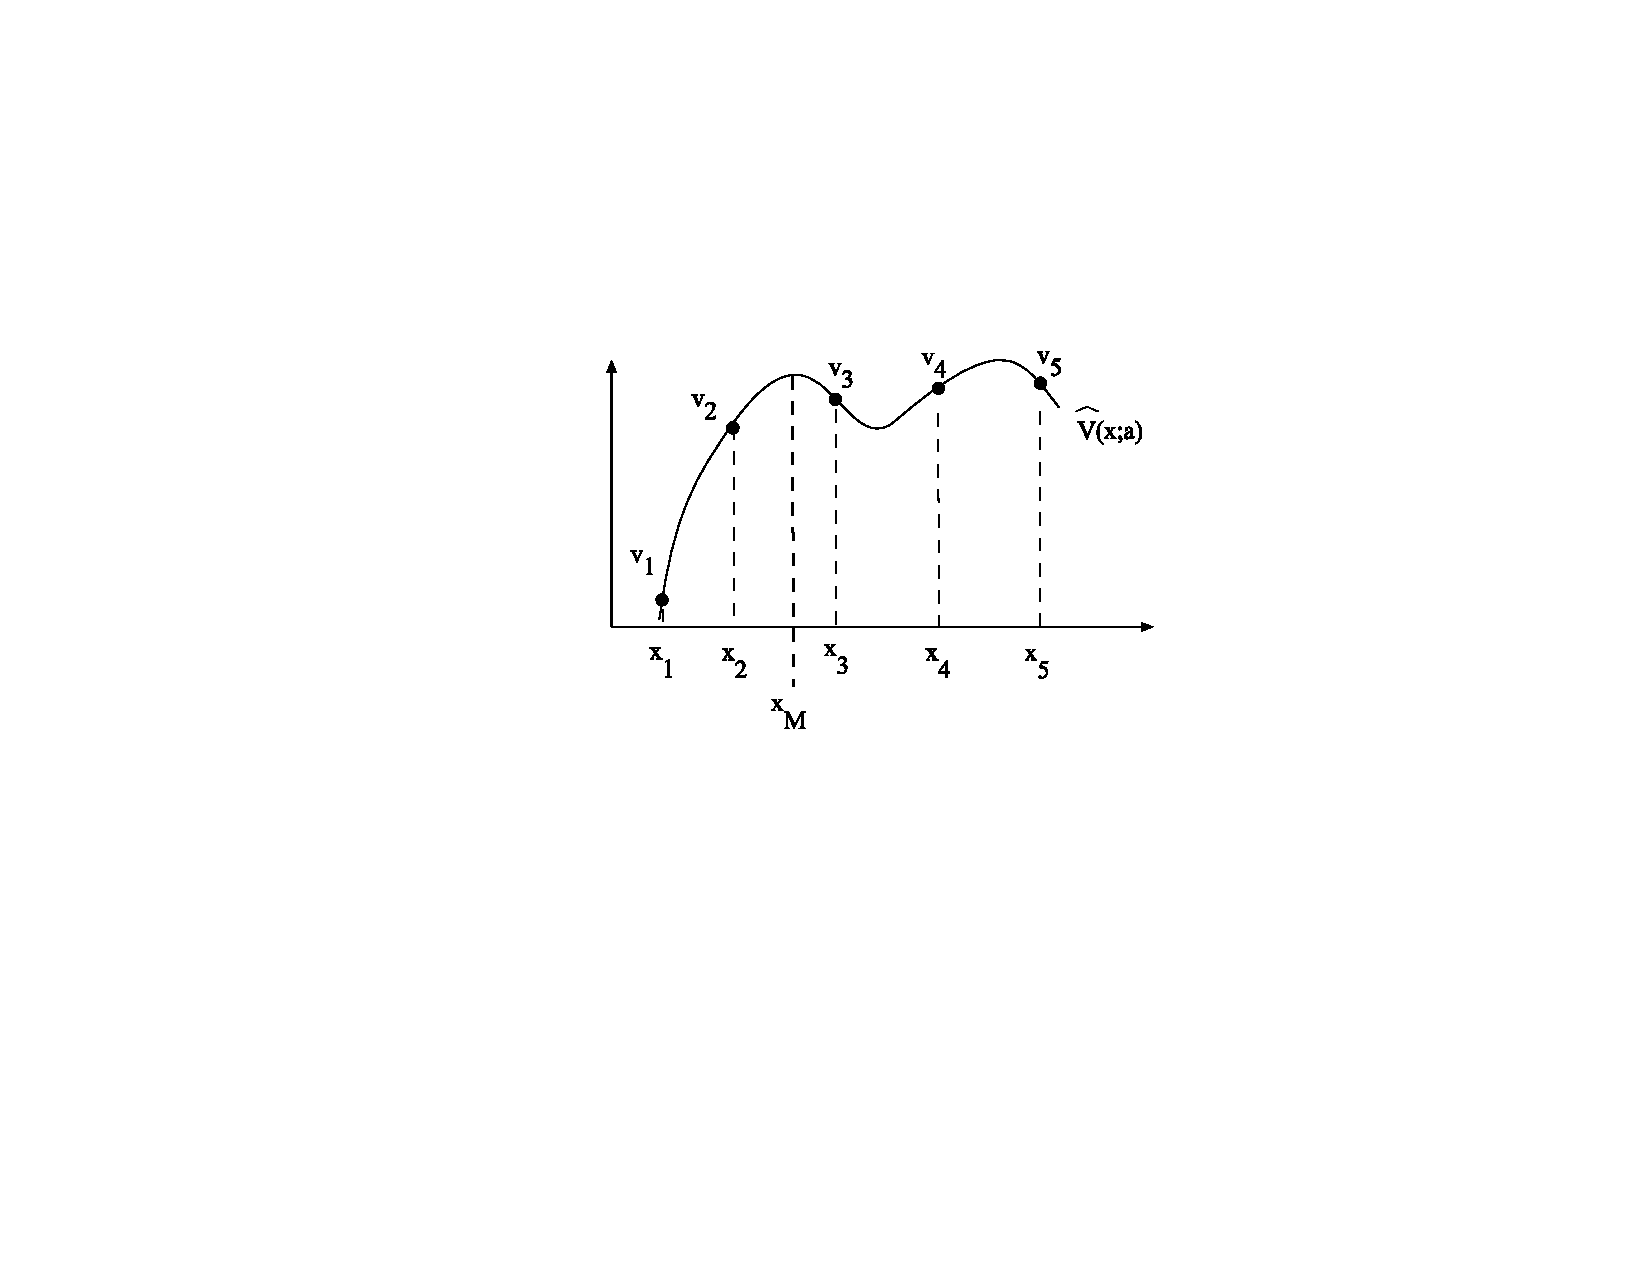
\includegraphics[height=2in]{./resources/spline_textbook.pdf}
\label{default}
\end{center}
\end{figure}
\begin{itemize}
\item Concave (monotone) data may lead to non concave (non monotone) approximations
\end{itemize}
\end{frame}

\begin{frame}{Schumaker Procedure (Shape Preserving Splines)}
\begin{enumerate}
\item Take level (and maybe slope) data at nodes $x_k$
\item Add intermediate nodes $z_k^{+} \in [x_k,x_{k+1}]$
\item Run quadratic spline with nodes at the $x$ and $z$ nodes which interpolate data and preserves shape
\item Schumaker formulas tell you how to choose the $z$ and spline coefficient
\item Detail in Judd and in companion paper (Judd and Solnick)
\end{enumerate}
\end{frame}

\begin{frame}[fragile]{Spline Example}
\begin{columns}
\begin{column}{0.5\textwidth}
\begin{itemize}
\item Try two piecewise cubics (at $x=3$)
\item Try three piecewise cubics (at $x=(2,4)$)
\item Try single cubic
\end{itemize}

 \tiny
 \vspace{2.4cm}
\begin{verbatim}
library(splines)
ggplot(data=NULL,aes(x, y)) + geom_point() + 
  geom_smooth(method = "lm", formula = y ~ bs(x,knots=3) ,color='maroon')+
  geom_smooth(method = "lm", formula = y ~ bs(x,knots=c(2,4)) ,color='darkgreen')+
  geom_smooth(method = "lm", formula = y ~ poly(x, 3),color='navy')
\end{verbatim}
\end{column}
\begin{column}{0.5\textwidth}  %%<--- here
    \begin{center}
    
\includegraphics[width=\textwidth]{./resources/splines.pdf}
     \end{center}
\end{column}
\end{columns}
\end{frame}



\begin{frame}[fragile]{Spline Example}
\begin{itemize}
\item Alternative is to use \alert{generalized additive model} and fit a spline with the \texttt{s()} function.
\item These can be made quite flexible (but this is simple).
\end{itemize}
 \tiny
\begin{verbatim}
library(mgcv)
ggplot(data=NULL,aes(x, y)) + geom_point() + 
  geom_smooth(method = "lm", formula = y ~ bs(x,knots=3) ,color='maroon')+
  stat_smooth(method = gam, formula = y ~ s(x),color='navy')
\end{verbatim}
\end{frame}


  
  
\begin{frame}{My own example}
\begin{center}
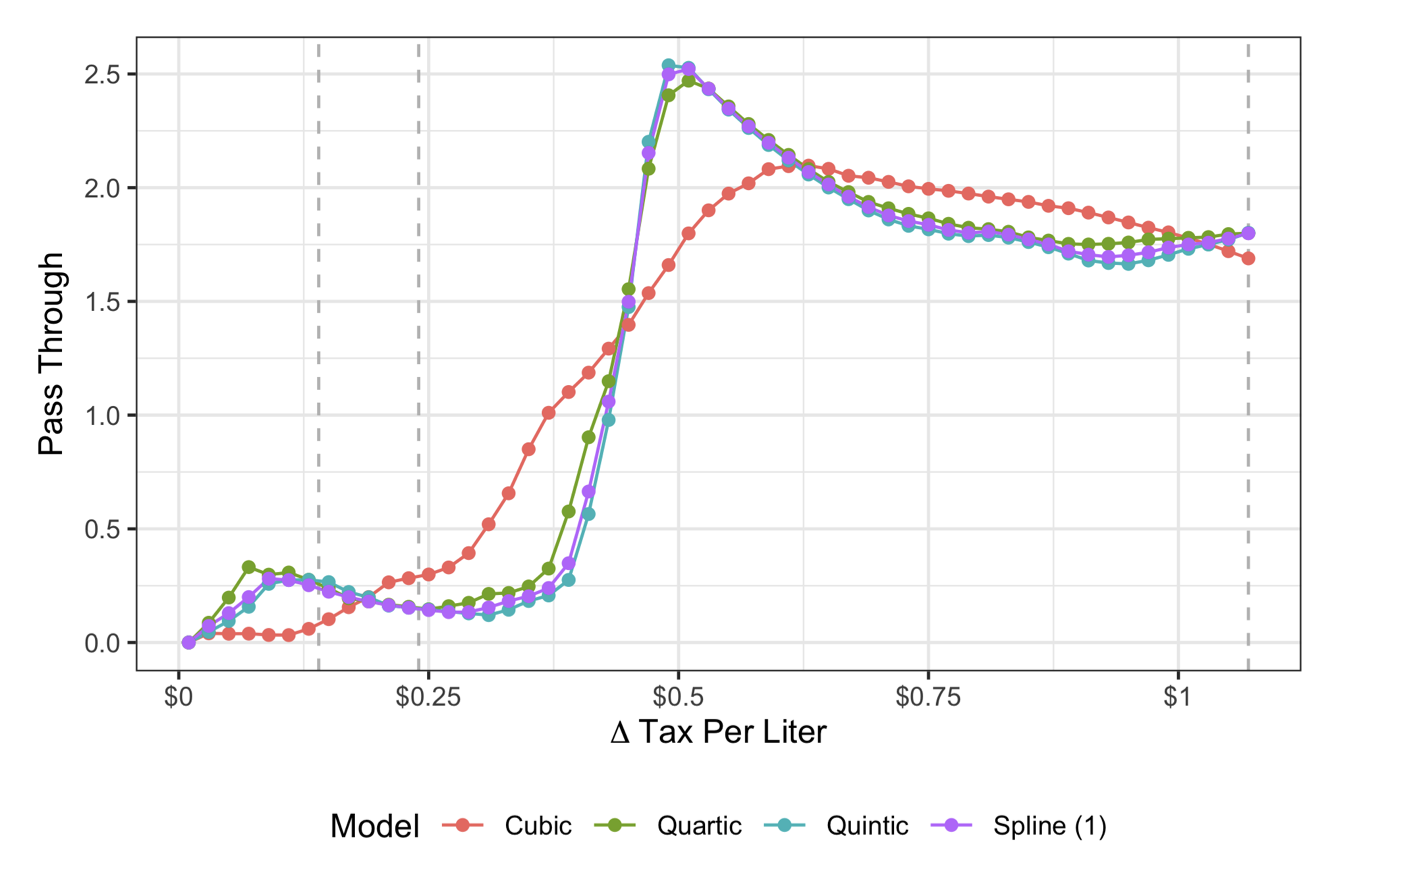
\includegraphics[height=0.8\textheight]{./resources/ptr.png}\\
Cubic isn't flexible enough, spline and quartic look about the same.
\end{center}
\end{frame}



\end{document}